\documentclass[aps,prl,reprint,amsmath]{revtex4-2}

\usepackage{graphicx}

\begin{document}

\title{Correcting K-correction: dark energy is based on a math error from 1930}

\author{Logan P. Evans}
 \email{loganpevans@gmail.com}
 \noaffiliation

\date{\today}

\begin{abstract}
We rederive the K-correction equation and discover that the version commonly
used to calculate magnitudes contains multiple errors. The oldest of these
errors traces back to 1930 and two new errors were introduced in 1996. We
conclude that properly correcting apparent magnitudes for redshift resolves two
of the preeminent mysteries in cosmology: first, dark energy is not supported
by observations of Type Ia supernovae and second, the Hubble tension is due to
the errors in the K-correction equation.
\end{abstract}

\maketitle

\section{Introduction}

The estimate of Type Ia supernovae (SnIa) distances is one of the primary
sources of data for cosmological models. Performing these distance estimates
involves taking a measurement of redshifted light in our observation frame and
then calculating the rest frame magnitude as if no redshift had occurred. The
equation that converts from an observation frame magnitude to a rest frame
magnitude is called K-correction.

\citet{tolman1930} published the first formal derivation of K-correction, but
he did not account for spectral bandwidth stretching, one of the dimming
effects of redshift. An alternative K-correction was correctly derived by
\citet{desitter1934}. However, in \citet{hubble1935}, the discrepancy was
briefly discussed yet dismissed. \citet{oke1968} rederived the K-correction
equation where they accounted for spectral bandwidth stretching, but they did
not account for time dilation, one of the other dimming effects of redshift.
The paper by \citet{kim1996}, which is the basis for modern implementations of
K-correction, extended the work of \citet{oke1968} to handle additional
cross-filter comparisons and added a term that was intended to address
zero-point corrections. This history is explored in more depth in Section
\ref{sec:history}.

The effect of using an incorrect redshift correction for SnIa is that we think
objects are farther away than they really are; this effect compounds for
greater distances. Up until \citet{riess1998}, we did not have distant enough
observations for this error to matter much for cosmological models, but by the
late 1990s, it became clear that our measurements for distance and redshift
were not linear. This realization led to a model that utilized a cosmological
constant $\Lambda$ and dark energy in order to explain the non-linear
distance-redshift graph. We will show in Section \ref{sec:conclusions} that
correcting the flaws of K-correction leads to a linear graph that does not
need to rely on a cosmological constant.

\citet{planck2015} used an alternative technique to compute the Hubble constant
$H_0$ that is based on measurements of the cosmic microwave background (CMB).
CMB-based computations of $H_0$ have made it evident that something is missing
with our understanding of cosmology because this technique produces a
significantly different value than when the constant is derived using SnIa.  As
we will discuss in Section \ref{sec:conclusions}, fixing the errors with
K-correction produces a measurement of the Hubble constant that is compatible
with models based on the CMB.

\section{A brief history of K-correction}
\label{sec:history}

Observational data from SnIa are essential for the calibration of models that
use redshift to estimate distance. The approximately linear relationship
between redshift and luminosity distance, often called the Hubble-Lema\^{i}tre law,
describes how quickly the universe is expanding. However, \citet{riess1998}
and \citet{perlmutter1999} presented evidence that there is not a linear
relationship between redshift and distance, but instead, distant objects are
farther away than their redshift would predict (see Figure
\ref{fig:mu_distance_vs_redshift}). This phenomenon implies that the
acceleration of the universe is faster today than it was for old observations.
The cause of this phenomenon was unknown and was referred to as dark energy.

\begin{figure}
  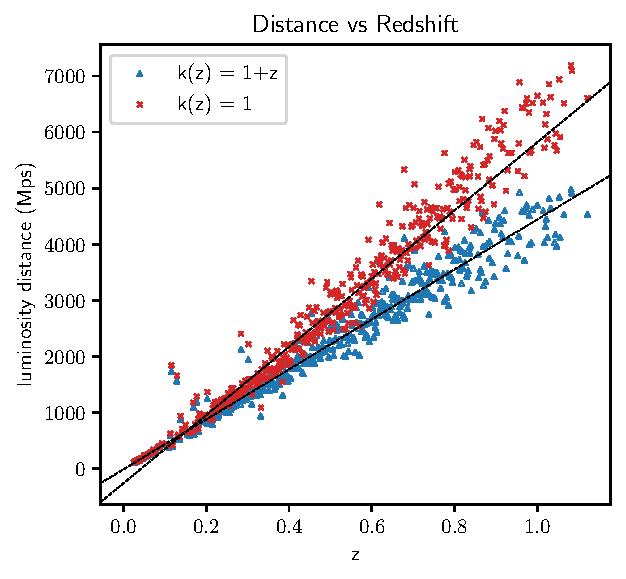
\includegraphics[width=\columnwidth]{lum_distance_vs_redshift.pdf}
  \caption{The relationship between luminosity distance and redshift for two
  treatments of the magnitude data. The red $k(z) = 1$ treatment, which represents
  the uncorrected values, is clearly non-linear while the blue $k(z) = 1 + z$
  treatment, which fixes the K-correction redshift error, appears to be linear.
  The displayed points are roughly a third of the values in the full SnIa
  dataset published in \citet{abbott2024}, selected with uniform redshift
  spacing to aid visibility. }
  \label{fig:mu_distance_vs_redshift}
\end{figure}

SnIa are used to explore the relationship between distance and redshift because
these events have a roughly constant absolute magnitude, which allows us to use
the apparent magnitude to estimate distance. An analogy is to imagine someone
walking in the dark and lighting matches. If we know how brightly a match burns
at a known distance, we can estimate the distance to any match by measuring the
apparent brightness before applying some geometry.

However, redshifting dims the luminosity of an observation in three ways:

\begin{itemize}
  \item The energy of a wave is inversely proportional to its wavelength; thus a
  redshift of $z$ means the amount of energy per photon is reduced by a factor
  of $1 / (1+z)$.

  \item The bandwidth stretches. If the rest frame observes photons in the
  bandwidth from 400nm and 401nm, then a redshift of $z = 1$ stretches the
  wavelengths to the bandwidth from 800nm to 802nm. The number of photons per
  bandwidth is reduced by a factor of $1 / (1+z)$.

  \item Cosmological time dilation reduces the rate at which photons arrive.
  The number of photons that arive per second is reduced by a factor of $1 / (1+z)$.
\end{itemize}

To complicate matters, we use the $B$ band magnitude to calculate luminosity
distance. We want to know how bright a supernova appears for wavelengths around
445nm as if no redshift had occurred. However, we typically need to observe the
supernova with a filter that is sensitive to longer wavelengths, such as the
$i$ band filter which is sensitive to wavelengths from 700nm-850nm
\citep{flaugher2015}. The K-correction formula allows us to take a magnitude
measured in an observation filter $y$ and compute the magnitude in the target
filter $x$.

The first mathematical treatment of K-correction was performed by
\citet{tolman1930}. However, when Tolman made his derivation, he did not
consider the effects of a spectrum that is stretched due to redshift.

A few years later, \citet{desitter1934} discussed all three issues that reduce
the observed magnitude of a distant observation. The correction for each of
these issues is identical: take a measurement for luminosity and multiply it by
the factor $1 + z$.

A year later, \citet{hubble1935} published a similar set of calculations where they noted:

\begin{quote}
It should be specially noted that this expression differs from the correction
to $m$ proposed by de Sitter, which contains the term $(1 + z)^3$ instead of
$(1 + z)^2$. Expression (28), however, would seem to give the proper correction
to use in connection with our equation (21), since it has been derived in such
a way as to make appropriate allowance, first, for the double effect of nebular
recession in reducing both the individual energy and the rate of arrival of
photons, and then for the further circumstance that a change in spectral
distribution of the energy that does arrive will lead to changes in its
photographic effectiveness.
\end{quote}

\noindent However, even though they considered all three dimming effects of
redshift, they started their derivation by copying the incorrect equation from
1930. The incorrect correction term has been used ever since.

In a paper published by \citet{oke1968}, the two factors of $(1 + z)$ were
attributed to the change in energy and to the spectral bandwidth elongation,
which leaves time dilation as the factor that was omitted.

The modern treatment of K-correction is based on the work of \citet{kim1996}.
This work extended the work of \citet{oke1968} to apply to filters beyond the
blue $B$ and visible $V$ bands. It also introduced a term that deals with the
zero-point for the actual filters. Historically, bolometric devices would
measure the energy flux, but modern charge-coupled device (CCD) cameras
effectively measure the photon flux, so \citet{kim1996} derived a form of the
K-correction equation that uses photon flux.

Quoting \citet{kim1996}:

\begin{quote}
  Therefore, the correct K correction calculation to be used with measured
  photometric magnitudes is the integral photon counts:

  \begin{equation}
  \begin{aligned}
  \label{eq:kim}
    K_{xy} =
      &-2.5\text{log} \left(
        \frac{\int \lambda \mathcal{Z}(\lambda)S_x(\lambda)d\lambda}
             {\int \lambda \mathcal{Z}(\lambda)S_y(\lambda)d\lambda}\right) \\
      &+ 2.5\text{log}(1+z) \\
      &+ 2.5\text{log}\left(
        \frac{\int \lambda F(\lambda)S_x(\lambda)d\lambda}
             {\int \lambda F(\lambda/(1+z))S_y(\lambda))d\lambda}\right).
  \end{aligned}
  \end{equation}
\end{quote}

This equation has three errors that we will explore in Section
\ref{sec:consequences}.

\section{Derivation of K-correction}
\label{sec:derivation}

The K-correction $K_{xy}$ uses a spectral energy density $F$ template that
specifies the expected spectrum for a SnIa observation. It also uses the
observed redshift $z$ and the observed photon flux magnitude $m_y$.

With modern CCD cameras, a telescope observation consists of a single value
$\mathcal{F}_y$ erg/s, which represents the energy collected per second in
filter $y$. Photogenerated electrons are collected in potential wells, which
means that the energy measured in this filter is proportional to the number of
photons \citep{lesser2015}. However, we need to calculate the expected number
of photons collected by using a spectral energy density function $F$.

\begin{figure}
  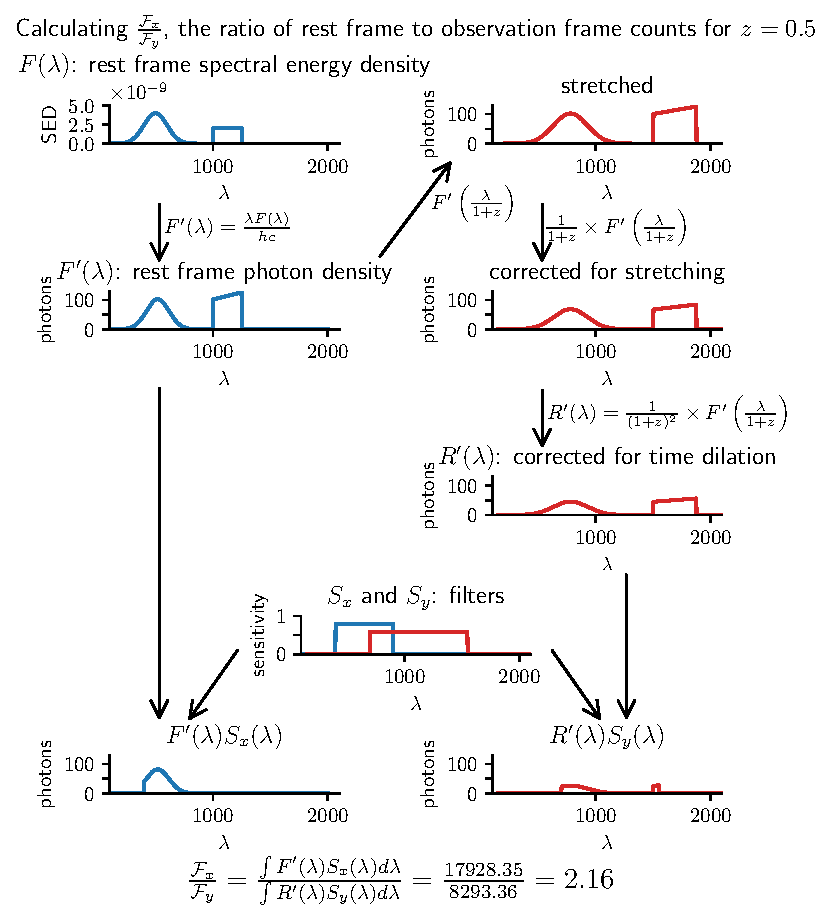
\includegraphics[width=\columnwidth]{k_equation_flow.pdf}
  \caption{The value $K'_{xy}$ is equal to the number of photons we want to
  report in the target filter divided by the number of photons we measure in
  the observation filter. Deriving this value starts with $F(\lambda)$, the
  spectral energy density, which we then convert to $F'(\lambda)$, the photon
  density for the rest frame. Starting at the top right corner of the figure we
  show three steps used to compute $R'(\lambda)$, the photon density in the
  observation frame. We first stretch the photon density, but this step
  inflates counts. In the second step, we correct for the inflated counts by
  multiplying by $1/(1+z)$; at this point, the total count equals the total
  count of $F'(\lambda)$. Finally, in the third step we finish calculating the
  observation frame photon density $R'(\lambda)$ by accounting for time
  dilation, which also reduces photon counts by a factor of $1/(1+z)$. We can
  compute the expected ratio of photons by totalling the area under the curves
  in the bottom two panels.
  }
  \label{fig:k-example}
\end{figure}

To convert the spectral energy density $F$ to the photon density $F'$, we need
to use the Plank relation $E = hc / \lambda$ where $E$ is the energy, $h$
is Planck's constant, and $c$ is the speed of light. This gives us

\begin{equation}
\begin{aligned}
   F(\lambda) &= F'(\lambda) \times \frac{hc}{\lambda} \\
  F'(\lambda) &= \frac{\lambda F(\lambda)}{hc}.
\end{aligned}
\end{equation}

It is important to note that for the blueshifted wavelength $\lambda / (1+z)$,
this equation produces

\begin{equation}
 F'\left(\frac{\lambda}{1+z}\right) = \frac{\lambda}{(1+z)hc} F\left(\frac{\lambda}{1+z}\right).
\end{equation}

\noindent However, this equation is misleading and error prone. We will want to
use it to help calculate the flux in an observation filter at the redshifted
wavelength $\lambda \times (1 + z)$. In other words, we want to produce the
photon density function $R'$ that is the redshifted version of $F'$.
Redshifting the photon density does two things:

\begin{itemize}
  \item All wavelengths are increased by a factor of $1 + z$. When we integrate
  $R'$ from wavelength $\lambda_a$ to wavelength $\lambda_b$, the values
  correspond to the wavelengths $\lambda_a / (1+z)$ to $\lambda_b / (1+z)$ in
  $F'$. We will integrate over a width of $\lambda_b - \lambda_a$, but
  $F'(\lambda / (1+z))$ will refer to values in a width of
  $(\lambda_b - \lambda_a) / (1+z)$.

  In order to account for the spectral bandwidth stretching effect, we
  multiply $F'$ by $1/(1+z)$.

  \item The stretching of space increases the distance between photons while
  they are traveling. To an observer, this phenomenon appears like time
  dilation, although cosmological time dilation is due to a different mechanism
  than relativistic time dilation. This effect reduces the photon arrival rate
  by a factor of $1/(1+z)$.

  In order to account for cosmological time dilation, we multiply $F'$ by a
  second factor of $1/(1+z)$.
\end{itemize}

Combining these two phenomena, we can calculate the redshifted spectral energy
density $R$ using

\begin{equation}
\begin{aligned}
\label{eq:redshifted_density}
  R'(\lambda) &= F'\left(\frac{\lambda}{1+z}\right) \times \frac{1}{(1 + z)^2} \\
  R(\lambda) &= \frac{\lambda}{(1+z)hc} \times F\left(\frac{\lambda}{1+z}\right) \times \frac{1}{(1 + z)^2} .
\end{aligned}
\end{equation}

\noindent We deliberately do not combine all of the factors of $1+z$ together because
this form is more natural to implement in code.

In order to calculate the flux $\mathcal{F}_x$ measured in filter $x$, we need
to compute the photon density $F'(\lambda)$ and multiply it by the sensitivity
$S_x(\lambda)$, which represents the proportion of photons with wavelength
$\lambda$ that filter $x$ will measure. We then sum over all wavelengths, which
is expressed with the equation

\begin{equation}
\begin{aligned}
\label{eq:flux_definition}
  \mathcal{F}_x &= \int F'(\lambda) S_x(\lambda) d\lambda \\
                &= \int \lambda F(\lambda) S_x(\lambda) d\lambda.
\end{aligned}
\end{equation}

We will also use the flux $\mathcal{F}$ to magnitude $m$ formula:

\begin{equation}
\begin{aligned}
\label{eq:flux2mag}
                             m_x &= -2.5 \text{log}(\mathcal{F}_x) + P_x \\
  -2.5 \text{log}(\mathcal{F}_x) &= m_x - P_x .
\end{aligned}
\end{equation}

\noindent $P_x$ represents the zero-point for the filter $x$ on some particular
telescope. In order to use consistent magnitude values across telescopes that
have different light gathering abilities, we take the measured magnitude and
multiply it by the ratio of the standard flux rate to the flux rate for this
particular telescope and filter. For convenience, we use $P_x = -2.5
\text{log}(P'_x)$ so that we can work with flux instead of with magnitude.

Now that we have the identities in Equations \ref{eq:flux_definition} and
\ref{eq:flux2mag}, we will change directions and look at the definition of
K-correction $K_{xy}$. This value allows us to make an observation in filter
$y$ and report what the magnitude would have been in filter $x$ if no redshift
occurred:

\begin{equation}
\begin{aligned}
\label{eq:definition}
  m_y &= M_x + \mu + K_{xy} \\
      &= M_x + m_x - M_x + K_{xy} \\
      &= m_x + K_{xy} \\
  m_x &= m_y - K_{xy} .
\end{aligned}
\end{equation}

\noindent The second line of Equation \ref{eq:definition} expands the distance modulus
$\mu$ using $\mu = m - M$ where $m$ is the observed magnitude and $M$ is the
absolute magnitude.

Since the K-correction is a magnitude value and we wish to work on flux values,
it is convenient to define the following substitution:

\begin{equation}
\label{eq:k_substitution}
  K_{xy} = 2.5\text{log}(K'_{xy}) .
\end{equation}

\noindent Note that this substitution omits the minus ($-$) sign that we used on a
similar substitution for $P_x$.

Starting with Equation \ref{eq:flux2mag} and then
recombining the flux term $\mathcal{F}_y$ with $m_y$ from Equation
\ref{eq:definition}, we have

\begin{equation}
\begin{aligned}
\label{eq:as_flux}
  -2.5 \text{log}(\mathcal{F}_x)
      &= m_x - P_x \\
      &= m_y - K_{xy} - P_x \\
      &= -2.5 \text{log}(\mathcal{F}_y) + P_y - K_{xy} - P_x \\
      &= -2.5 \text{log}(\mathcal{F}_y) \\
         &\qquad - 2.5 \text{log}(P'_y) \\
         &\qquad - 2.5 \text{log}(K'_{xy}) \\
         &\qquad + 2.5 \text{log}(P'_x) \\
      &= -2.5 \biggl(\text{log}(\mathcal{F}_y) + \text{log}(K'_{xy}) \\
         &\qquad\qquad + \text{log}(P'_y) - \text{log}(P'_x)
        \biggr) \\
      &= -2.5 \text{log}\left(
        \mathcal{F}_y
        \times K'_{xy}
        \times \frac{P'_y}{P'_x}\right) \\
  \mathcal{F}_x &= \mathcal{F}_y \times K'_{xy} \times \frac{P'_y}{P'_x}.
\end{aligned}
\end{equation}

\noindent We can isolate $K'_{xy}$ and then use Equation \ref{eq:flux_definition} to expand

\begin{equation}
\begin{aligned}
  \mathcal{F}_x &= \mathcal{F}_y \times K'_{xy} \times \frac{P'_y}{P'_x} \\
        K'_{xy} &= \frac{P'_x}{P'_y} \times \frac{\mathcal{F}_x}{\mathcal{F}_y} .
\end{aligned}
\end{equation}

\noindent We now use Equations \ref{eq:redshifted_density} and \ref{eq:flux_definition}
to calculate the fluxes $\mathcal{F}_x$ and $\mathcal{F}_y$ in terms of the
spectral energy density function $F$. Note that $\mathcal{F}_x$ uses the rest
frame spectral energy density $F$, while $\mathcal{F}_y$ uses the redshifted
spectral energy density $R(\lambda)$:

\begin{equation}
\begin{aligned}
  K'_{xy} &= \frac{P'_x}{P'_y} \times \frac{\mathcal{F}_x}{\mathcal{F}_y} \\
         &= \frac{P'_x}{P'_y} \times
              \frac{\int F'(\lambda) S_x(\lambda) d\lambda}
                   {\int R'(\lambda) S_y(\lambda) d\lambda} \\
         &= \frac{P'_x}{P'_y} \times
              \frac{\int F'(\lambda) S_x(\lambda) d\lambda}
                   {\int F'\left(\frac{\lambda}{1+z}\right) \times \left(\frac{1}{1 + z}\right)^2 S_y(\lambda) d\lambda} \\
         &= \frac{P'_x}{P'_y} \times (1+z)^2 \times
              \frac{\int \left(\frac{\lambda}{hc}\right) F(\lambda) S_x(\lambda) d\lambda}
                   {\int \left(\frac{\lambda}{(1+z)hc}\right) F\left(\frac{\lambda}{1+z}\right) S_y(\lambda) d\lambda} \\
         &= \frac{P'_x}{P'_y} \times (1 + z)^2 \times
              \frac{\int \lambda F(\lambda) S_x(\lambda) d\lambda}
                   {\int \left(\frac{\lambda}{1+z}\right) F\left(\frac{\lambda}{1+z}\right) S_y(\lambda) d\lambda} .
\end{aligned}
\end{equation}

Finally, we use Equation \ref{eq:k_substitution} to convert $K'_{xy}$ back into
the magnitude $K_{xy}$:

\begin{equation}
\begin{aligned}
\label{eq:K2k}
  K_{xy} &= 2.5\text{log}(K'_{xy}) \\
         &= 2.5\text{log}\left(
            \frac{P'_x}{P'_y} \times (1 + z)^2 \times
            \frac{\int \lambda F(\lambda) S_x(\lambda) d\lambda}
                 {\int (\lambda / (1+z)) F(\lambda / (1+z)) S_y(\lambda) d\lambda}\right) \\
         &= 2.5 \left(
            \text{log} \left( \frac{P'_x}{P'_y} \right)
            + \text{log}( {(1 + z)^2})
            + \text{log}\left( \frac{\int \lambda F(\lambda) S_x(\lambda) d\lambda}
                                    {\int (\lambda / (1+z)) F((\lambda)/ (1+z)) S_y(\lambda) d\lambda}
            \right) \right) \\
         &= 2.5 \text{log} \left( \frac{P'_x}{P'_y} \right)
            + 5 \text{log} (1 + z)
            + 2.5 \text{log} \left(
              \frac{\int \lambda F(\lambda) S_x(\lambda) d\lambda}
                   {\int (\lambda / (1+z)) F(\lambda / (1+z)) S_y(\lambda) d\lambda} \right) \\
         &= 5 \text{log} (1 + z)
            + 2.5 \text{log} \left(
              \frac{\int \lambda F(\lambda) S_x(\lambda) d\lambda}
                   {\int (\lambda / (1+z)) F(\lambda / (1+z)) S_y(\lambda) d\lambda} \right)
            - P_x + P_y .
\end{aligned}
\end{equation}

\section{Consequences}
\label{sec:consequences}

In order to fully compare our derivation against Equation \ref{eq:kim} (from
\citet{kim1996}) we need to use the identity

\begin{equation}
  P = -2.5 \text{log} \left( \int \frac{\lambda}{hc} \mathcal{Z}(\lambda) S(\lambda) d\lambda \right)
\end{equation}

\noindent where, according to \citet{kim1996}, ``$\mathcal{Z}(\lambda)$ is an
idealized spectral energy distribution at $z = 0$ for which
$U = B = V = R = I = 0$ in the photometric system being used.'' Combining this
with Equation \ref{eq:K2k}, we have

\begin{equation}
\begin{aligned}
  K_{xy} &= 5 \text{log} (1 + z)
            + 2.5 \text{log} \left(
              \frac{\int \lambda F(\lambda) S_x(\lambda) d\lambda}
                   {\int (\lambda / (1+z)) F(\lambda / (1+z)) S_y(\lambda) d\lambda} \right)
            - P_x + P_y \\
         &= 5 \text{log} (1 + z)
            + 2.5 \text{log} \left(
              \frac{\int \lambda F(\lambda) S_x(\lambda) d\lambda}
                   {\int (\lambda / (1+z)) F(\lambda / (1+z)) S_y(\lambda) d\lambda} \right) \\ &\ \ \
            + 2.5 \text{log} \left( \int (\lambda / hc) \mathcal{Z}(\lambda) S_x(\lambda) d\lambda \right)
            - 2.5 \text{log} \left( \int (\lambda / hc) \mathcal{Z}(\lambda) S_y(\lambda) d\lambda \right) \\
         &= 2.5 \text{log} \left(
              \frac{\int \lambda \mathcal{Z}(\lambda) S_x(\lambda) d\lambda}
                   {\int \lambda \mathcal{Z}(\lambda) S_y(\lambda) d\lambda}
             \right)
            + 5 \text{log} (1 + z)
            + 2.5 \text{log} \left(
              \frac{\int \lambda F(\lambda) S_x(\lambda) d\lambda}
                   {\int (\lambda / (1+z)) F(\lambda / (1+z)) S_y(\lambda) d\lambda} \right) .
\end{aligned}
\end{equation}

Three differences with Equation \ref{eq:kim} stand out:

\begin{itemize}
  \item The sign is different for the first term. This will have a subtle but
  frustrating effect for real measurements. The zero-point values for the two
  filters are usually, but not always, roughly equal. As we observe more
  distant supernovae, it is useful to switch our observational filter to a
  filter that is sensitive to longer wavelengths, but each observation filter will
  have its own small bias.

  \item The second term is multiplied by $2.5$ in \citet{kim1996}, but is
  multiplied by $5$ here. This is the manifestation of the error in
  \citet{tolman1930} and leads to the conclusion that the expansion of the
  universe is accelerating.

  \item In our derivation, the third term has an extra $1 + z$ expression.
  Based on an inspection of the SN(oo)py software package presented by
  \citet{burns2010} and the SNANA software package presented by
  \citet{kessler2009}, this error is ignored and software package authors
  implement it as intended, not precisely as written.
\end{itemize}

\section{Conclusions}
\label{sec:conclusions}

\begin{figure}
  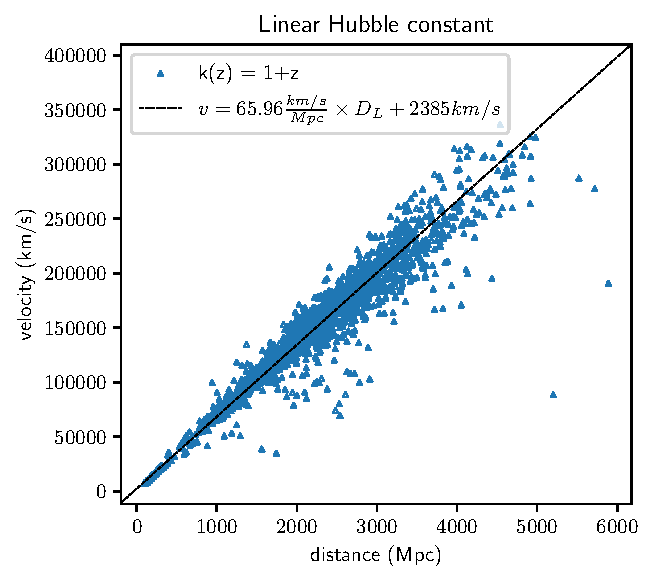
\includegraphics[width=\columnwidth]{velocity_vs_distance.pdf}
  \caption{The relationship between expansion velocity and distance. The slope
  of this graph demonstrates the Hubble constant. The data for these SnIa
  observations comes from the Dark Energy Survey \citep{vincenzi2024}, but the
  magnitudes are corrected to account for time dilation by adding
  $-2.5 log(1 + z)$.
  }
\label{fig:expansion}
\end{figure}

As shown in Figure \ref{fig:mu_distance_vs_redshift}, when reported magnitudes
are corrected by adding the magnitude $-2.5\text{log}(1+z)$, there is a linear
relationship between redshift and luminosity distance. This is in accordance
with the Hubble-Lema\^{i}tre law. As opposed to the uncorrected values, there
is no visual acceleration. Since the corrected values are approximately linear,
we can use them to estimate the Hubble constant $H_0$ which is demonstrated in
Figure \ref{fig:expansion}.

The value estimated here, $H_0 = 65.94 \pm 1.3$ is highly suspicious
because of the flipped zero-point corrections, but it is consistent with
estimates of $H_0$ that are based on the CMB. \citet{planck2020} published the
CMB value of $H_0 = 67.27 \pm 0.6$, and the one sigma error bars overlap. It
is interesting to note that restricting the Dark Energy Survey observations of
SnIa \citep{vincenzi2024} to only those with $z < 0.1$, which presumably is a
small enough redshift that most of the observations will have been made with
the same filter, gives the estimate $H_0 = 67.8 \pm 1.9$.

Since the K-correction error has corrupted all astronomical measurements that
depend on both magnitude and redshift, a lot of data needs to be reanalysed.
Cosmological parameters, such as those used by the
Friedmann-Lema\^{i}tre-Robertson-Walker (FLRW) metric or the $\Lambda$-CDM
model, can only be recalculated once the data is cleaned.

The reasons that the K-correction errors went undiscovered for so long should
also be explored. Many hints existed that something was wrong, yet the
problems persisted.

\bibliography{references}{}
\bibliographystyle{aasjournal}

\end{document}
